%!TEX root = ./intern_report.tex

\newpage
\subsection{Designing and Implementing an Efficient End-toEnd Pipeline for Machine Learning in Robotics}

\subsubsection{Need for a standard ML pipeline in DATA61}

\paragraph{}
Robotics and Autonomous Systems Group of CSIRO's DATA61 consists of world class engineers who have specialized in field robotics. Over their multiple years of experience in research and engineering, each of them have formulated an efficient workflow for themselves. Workflow is the general procedure where they collect data, process them in specialized software or write programs for custom processing, build software that can run real time on an existing robot to process the environment and make decisions, debugging their products or code and so on. 

\paragraph{}
Today, with the rise of machine learning in several fields, it is a valuable tool for a field roboticist since it is fundamentally suitable to address the common problem in field robotics: processing complicated real world through noisy sensors and making high level decisions. Many of these leading roboticists have realized that and have already started using machine learning in their projects. However, in DATA61, so far, there is no unified framework that acts as a common ground to the different researchers working in different projects. Also, many of them currently use their local computers (powered by GPUs) for machine learning tasks out of habit and convenience, rather than utilizing the supercomputing resources available at CSIRO. And some of them who have figured out the procedure of using a supercomputer follow certain practices which are fine in local computers, but inefficent when done on supercomputers.

\paragraph{}
When Nicolas Hudson (our supervisor) took position in DATA61, he set out with the task of streamlining the machine learning (and other) procedures in DATA61 into unified frameworks, such that different researchers can work together, share their knowledge on a common ground and follow practices which are efficient and that maximize the utilization of the resources at disposal. One of the main motives behind such a task of streamlining is the DARPA Subterranean Competition (see: section \ref{ssec:darpa}) on which different groups of DATA61 will be working together for the next few years. 

\subsubsection{Pipeline: An Overview}

\paragraph{}
Therefore, we were requested to create an end to end pipeline for machine learning. This pipeline should be compliant with the current general workflow of most roboticists in RAG and should be efficient and scalable. We were asked to use the latest versions of software and the most general hardware controllers so that our pipeline can be effectively generalized. It is end-to-end in the sense that includes best practices in collecting and storing data, building models and training them with large volumes of data and finally deploying the trained models on power-constrained high level controllers which are to be mounted on robots.

\begin{figure}[H]
    \centering
    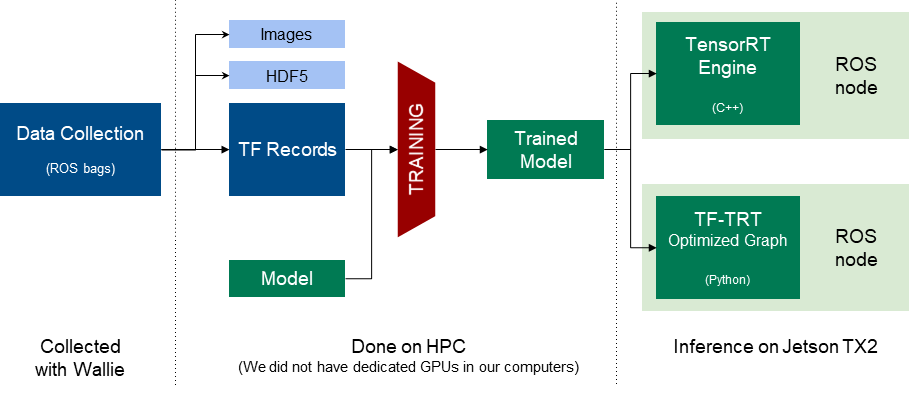
\includegraphics
        [width=16cm]
        {figures/full_pipeline.PNG}
    \caption{End-to-End Pipeline we built \label{Fig:pipeline}}\vspace{-4mm}
\end{figure}

\paragraph{}
We were asked to do the two projects: Trailnet and Hillnet using this pipeline while perfecting the pipeline itself as a proof of concept. We were also asked to document our processes extensively in the internal wiki pages of CSIRO along with reusable code. In addition we were requested to create simple code snippets that demonstrate the key points of each part of the pipeline and finally explain and demonstrate our pipeline to the fellow scientists at a Robotics Reading Group meeting.

\newpage
\subsubsection{Collecting and Storing Data}

\paragraph{}
In field robotics research, ROS (Robot Operating System) is used as the common platform or middleware to connect sensors and actuators of a robot. ROS packages are available for most of the professional high-end sensors and data from such sensors can be recorded in 'ROSbags'. ROSbag (.bag) is a file where all the activities of a ROS session was recorded in time-ordered format. They can be generated by a built in ros package. The user is able to record any session into a rosbag and play them later. ROS and ROSbags are used as the de-facto standard by the roboticists at CSIRO to collect data for analysis.

\paragraph{}
These ROSbags are unnecessarily huge in size and time-ordered. This poses difficulty in directly using them as a data storage format for machine learning. Due to their size, it is not possible to fit them into memory and due to their structure, it is not possible to perform multiple parallel reads from the same file in disk to accelerate the training process. Being time-ordered is an advantage for training RCNNs, but for training simple CNNs, we need the data to be completely shuffled for faster convergence when training.

\paragraph{}
\textbf{Storing as Images}

\paragraph{}
Therefore, the first solution is to generate a dataset of thousands of individual images (JPG, PNG) sorted into folders representing various classes. Such a dataset of images can be thoroughly shuffled easily, by simply shuffling a string-list of their filenames. Loading all the images into the memory at once is impossible even for 40,000 images. Instead, one can write scripts to read and queue images from disk, but it is cumbersome and error-prone. 

\paragraph{}
In addition to that, storing thousands of images in the HPC (High Performance Computing or Supercomputer) is highly discouraged. When it is done, the performance gains of processing the image faster is offset by the overhead delay of reading and processing the image headers of each JPG or PNG image and results in a slowdown. Also, storing a large 'number of files' in network drives puts a strain on the existing file management systems. I had my access revoked multiple times for accidentally storing a large number of files in my personal folders of the supercomputer.

\paragraph{}
\textbf{Storing as HDF files}

\paragraph{}
Due to these issues, I spent a few days experimenting with serialized file formats such as HDF5. They are ideal in the way that they are read from disk directly (not from memory) and queuing operations can be performed with little difficulty to boost the reading speed. However, a major problem with HDF files is the inability to render themselves to a shuffle operation. Since the data is serialized, to shuffle an existing HDF5 dataset, the entire dataset has to be read into the memory, which is impossible. Then the only solution is to shuffle before writing a dataset. But given that ROSbags can be read only in a time-ordered manner, this is also not possible.

\subsubsection{Storing as TF Records}

\paragraph{}
Then I turned to TF records, a dataset format recommended by the TensorFlow framework, which is the standard framework for ML in CSIRO RAG. I found TF records to be ideal for our purpose due to several reasons. Firstly, TFRecord is a serialized file format, that supports reading from disk. Also, the data stored in TFRecords can be bundled, like bundling attributes into an object in Object Oriented Programming. That is, the input image and the corresponding label, IMU data, velocity can all be bundled into a single TFexample, stored and retrieved for training. In addition to that, tensorflow offers multiple operations that can be performed on tfrecords to shuffle them, queue them and read them effectively without reading the entire file. In a nutshell, tfrecords were designed to be used in supercomputers and to solve the problems with other methods.


\begin{figure}[H]
    \centering
    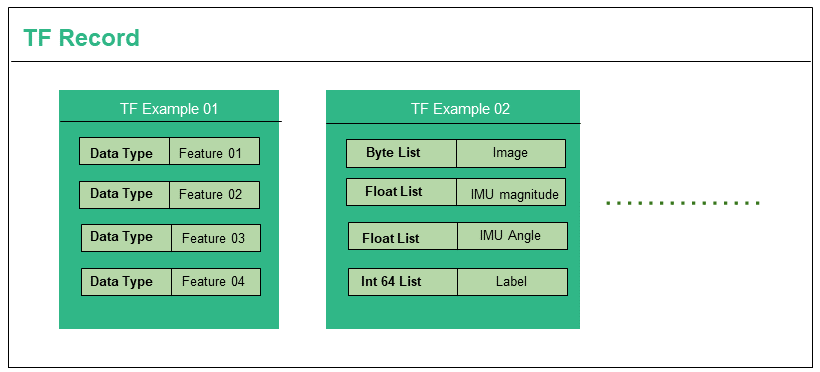
\includegraphics
        [width=9cm]
        {figures/tfrecord_structure.PNG}
    \caption{Structure of a TF Record}\vspace{-4mm}
\end{figure}

\newpage
\paragraph{}
A TFRecord dataset can be composed of thousands of tfexamples (tfexample is conceptually similar to an object in OOP, in reality is a protobuf defined in tensorflow). Each TFexample is a bundle of multiple features (a feature is conceptually similar to an attribute in OOP) that describe the TFexample. A feature can be of only one of three datatypes as allowed by tensorflow: ByteList, FloatList and Int64List. For efficient shuffling, one needs to split the dataset into multiple tfrecords. That is, as the raw file (such as ROSbag) is traversed in time-order, first 500 tfexamples should be written into one record in time-ordered manner, second 500 into next and so on. This is also because, having millions of examples inside one tfrecord slows down the read operation and the recommended optimum size of the tfrecord is around 100 MB.


\subsubsection{Training on Supercomputers}
\label{training_on_Supercomputers}

The set of tfrecords written that way can be read in the following manner. First, the list of tfrecord files in a dataset is shuffled. Then we start reading from all the tfrecords in parallel. Here, we can split the dataset into training and validation randomly. This read operation can be queued easily (prefetching). This pipeline can then be effectively shuffled (by shuffling files inside a prefetch buffer from each file and then interleaving them across the read heads from multiple files), repeated and decoded using a function we specify (to convert the tf datatypes to the datatypes we use, perform operations such as BGR to RGB conversion in images, changing dimensionality...etc), then batched and released as the input  for training a model.


\begin{figure}[H]
    \centering
    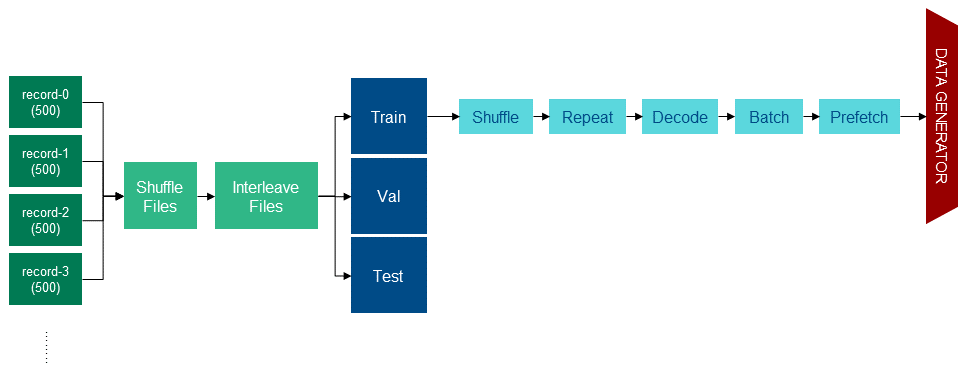
\includegraphics
        [width=16cm]
        {figures/input_pipeline.PNG}
    \caption{Data Input Pipeline with TFRecords for training}\vspace{-4mm}
\end{figure}

\paragraph{}
A key insight here is that each of the above mentioned operations: shuffle, interleave, decode, batch, prefetch, train-val split are all implemented as tensorflow ops (operations). That is, tensorflow follows a dataflow programming paradigm (like verilog HDL). We specify the operations that should be performed on data and the connections between those operations (a tensorflow graph) through our python code, but these operations are not performed as control flows through those respective lines in the code. Instead an abstract graph is formed as control flows through those statement. Finally, when we start a tensorflow session and run it (sess.run()), the graph gets executed and data starts flowing through it in parallel (much like verilog HDL). The above mentioned operations are also performed this way. We specify the transformations that should be done on the dataset in an abstract manner. Tensorflow forms a graph and performs those transformations in an efficient parallalized way that maximizes the use of resources at disposal.

\paragraph{}
TFRecords also yield well into the training of models in tensorflow and tensorflow-keras. Both APIs support generators, a type of python functions that mimic an iterator (like a list) to provide their input, output data pair for training. Such a generator can be created to read a set of tfrecords using the above ops and yield one pair at a time as output. This blends seamlessly into the training procedure. 


\paragraph{}
Unfortunately tfrecords are not very intuitive to use. Not many roboticists are not familiar with the unique datatypes and the dataflow programming paradigm of tensorflow. Advocating the use of tfrecords as the common dataset storage format and showing others how they can be included in their pre-established custom workflows was a key part in the development of the pipeline. I helped many of my coworkers by creating tools to visualize, write and read tfrecords. I also documented these procedures extensively for the future reference in CSIRO's wiki pages.


\newpage
\subsubsection{TensorRT: Deployment on a low power device}
\label{tensorrt}

\paragraph{}
Machine learning frameworks such as TensorFlow and Caffe are built to be optimized for training a neural network model. They use high precision datatypes and typically utilize a large amount of memory, GPU and processing resources even to perform inference using a trained model. In addition, neural networks are typically built and trained by data scientists without a software engineering background who prefer high level languages like python and generally are not focused on writing fast, efficient code to be run on resource-limited devices. This poses a key problem in machine learning: these models are generally not portable to devices that have limited memory, processing power and use little power. 

\begin{figure}[H]
    \centering
    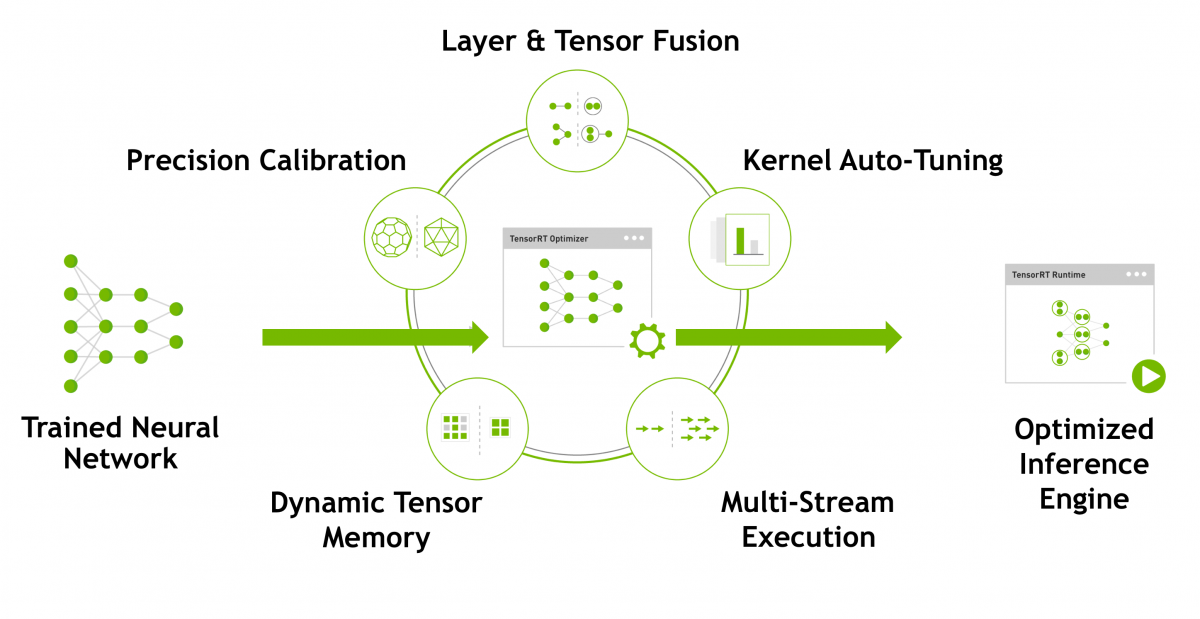
\includegraphics
        [width=13cm]
        {figures/trt.png}
    \caption{TensorRT in a nutshell}\vspace{-4mm}
\end{figure}

\paragraph{}
To address this problem, NVIDIA released TensorRT as their own library. TensorRT is NVIDIA's programmable inference accelerator, that can optimize any supported model for inference on devices with limited resources. When a model is optimized, first the full-precision float32 datatype is converted to half-precision float16. Then, tensorRT traverses the tensorflow graph and finds subgraphs that can be optimized. That is, a convolution operation followed by activation and max-pooling operations is combined into a single tensorRT operation that can be executed in very few clock cycles. These tensorRT operations are then assigned to various parts of the target device: the CPU, GPU and special DLA (Deep Learning Accelerator) chips and queued for parallel operation.

\paragraph{}
Therefore, by converting a tensorflow graph (optimized for training) into tensorRT graph (optimized for inference), one can obtain a model that can have very low latency during inference, used very little memory without a significant loss of accuracy. This model can then be deployed for inference on NVIDIA's embedded hardware such as Jetson TX2.

\paragraph{}
TensorRT is released both as a C++ API and a Python API. However, Jetson TX2 only supports the C++ API of TensorRT. The following figure shows the procedure I followed to convert a tensorflow graph into a tensorRT graph for inference. After conversion, I created C++ ROS nodes for Trailnet and Hillnet to accept messages from sensors, process them with the model and output velocity commands for the motor controller. The C++ API is extremely fast: it could process a 320 x 180 x 3 image through a resnet with 20 convolution layers within 5 ms, allowing a processing rate upto 200 frames per second.

\begin{figure}[H]
    \centering
    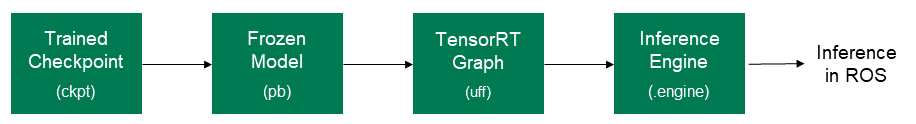
\includegraphics
        [width=13cm]
        {figures/deploy_pipeline_python.PNG}
    \caption{Deployment Pipeline: C++}\vspace{-4mm}
\end{figure}

\paragraph{}
However, not all models can be converted into tensorRT graphs for inference. That is, only a small subset of tensorflow's operations are supported by tensorRT for inference. For example, batch normalization, a common operation used in many networks, was not supported in tensorRT 3.0. Therefore, in order for our pipeline to be generalized, I also looked into a way to convert optimize any tensorflow graph for inference. Google and NVIDIA joined hands to solve this issue and have provided tensorflow-tensorRT (TF-TRT) as a part of tensorflow framework since 2017. TF-TRT can analyse any tensorflow graph (any neural network) and choose the subgraphs (operations) that can be accelerated by tensorRT. The unsupported operations are then perform through tensorflow in an unoptimized manner. Result is a model that is slower than pure tensorRT and faster than pure tensorflow during inference. Following is the workflow for this. 

\begin{figure}[H]
    \centering
    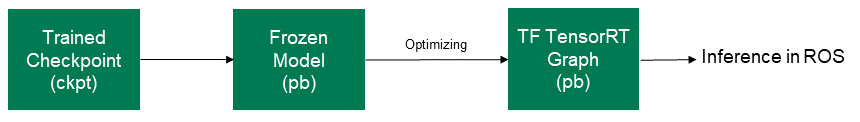
\includegraphics
        [width=13cm]
        {figures/deploy_pipeline_cpp.PNG}
    \caption{Deployment Pipeline: Python}\vspace{-4mm}
\end{figure}

\paragraph{}
I created a python ROS node also to accept messages from sensors, process them with the model and output velocity commands for the motor controller. The same network had a latency of 20 ms in the python node. That is about 50 frames per second. The detailed procedure and my scripts used for these conversions were documented thoroughly in CSIRO's wiki pages. 



\subsubsection{Problems Faced and Solutions}

\paragraph{}
When I began building the pipeline, the major problem I faced was that none of my coworkers were familiar with tfrecords. I had questions about the best practices in shuffling and the order of operations, which adequate answers were not provided in the documentation. Therefore, I started to experiment with a simple dataset of integers from 1 to 50,000. I brainstormed my ideas and tried different configurations of writing, reading and shuffling and figured out the best way of doing it efficiently.

\paragraph{}
Then, there was a problem when we found ROS was not installed on the supercomputer as a package and we are not allowed to install new packages there. This meant that we cannot play the ROSbags to extract them in the supercomputer. We tried to extract the ROSbags into tfrecords and then pushing the tfrecords into the supercomputer, but it was a cumbersome task and the storage on our local machines were not sufficient for that. Our coworker Micheal gave me a docker container image he has built for a similar task. Docker container is a virtual environment which one could build with necessary packages and run on a computer as an abstract layer. I spent several days building and rebuilding a docker based on that, to include rosbag, opencv and cvbridge python packages and used it to convert ROSbags to tfrecords in the supercomputer, without running ROS. 

\paragraph{}
When working with the C++ interface of tensorRT, I worked overnight at office to build the first draft of the ROS node: the pipeline to process the image and perform inference and faced with a TensorRT error: "dimensions don't match for the inputs of add layer". I spent a week debugging this issue: raised an issue in NVIDIA's developer forum, rechecking dimensions of my network, building a residual block with pure tensorflow ops and the problem persisted. I decided it was a bug.  After a week they confirmed it indeed was a bug and asked me to update our software to the latest version released few weeks prior to that. We did, and hence solved that issue.